\documentclass[a4paper]{article}
%\usepackage[english]{babel}
\usepackage{graphicx}
%\usepackage{multicol}
%\usepackage{amsmath}
%\usepackage{scrextend}
%\usepackage[colorinlistoftodos]{todonotes}
%\usepackage{blindtext}
%\newcommand*{\Scale}[2][4]{\scalebox{#1}{$#2$}}%
%\newcommand*{\Resize}[2]{\resizebox{#1}{!}{$#2$}}%
\usepackage{enumitem}
\usepackage{listingsutf8}
%\usepackage{listings}
%\usepackage{soul}
%\usepackage{float}
%\usepackage{epstopdf}
%\usepackage{subfig}
%\usepackage{amssymb}
%\setlist{leftmargin=5.5mm}
%\usepackage[all]{xy}
%\usepackage{pdflscape}
%\usepackage{longtable} 
%\usepackage{cite}
%\usepackage[hyphens]{url}
\usepackage[hidelinks]{hyperref}
%\hypersetup{breaklinks=true}
%\urlstyle{same}
\newcommand{\HRule}{\rule{\linewidth}{0.5mm}}
%\usepackage{pythonhighlight}
\usepackage{xcolor} %pas toucher du tout

%\pagecolor[rgb]{0,0,0} %black
%\color[rgb]{0.4,0.4,0.4} %white


\usepackage[acronym]{glossaries}
\makeglossaries
\newglossaryentry{dhcp}{name=DHCP,description={Le Dynamic Host Configuration Protocol est un protocole côté serveur et machine cliente qui permet de fournir des informations de configuration pour rejoindre un réseau local à une machine par l'envoi d'une réponse d'un serveur DHCP à une requête d'une machine cliente}}
\newglossaryentry{nat}{name=NAT,description={Un service de Network Address Translation ou de translation d'adresses réseau permet de faire correspondre des adresses IP d'un réseau à d'autres réseaux en traduisant les adresses d'un réseau local en une adresse publique du routeur vue par un ou des autres réseaux}}
\newglossaryentry{rpi}{name=Raspberry Pi, description={Un Raspberry Pi est un micro-ordinateur sous forme d'une carte informatique utilisable comme un ordinateur classique permettant notamment la manipulation plus facile d'appareils électronique}}
\newglossaryentry{rpios}{name=Raspberry Pi OS, description={Le système d'exploitation Raspberry Pi OS est developpé par l'équipe de Raspberry afin d'être installé et d'être utilisé sur leur micro-ordinateurs Raspberry Pi}}
\newglossaryentry{ipforward}{name=IP forward, description={L'IP Forward est un principe de routage de paquets IP permettant la redirection de paquets sur une interface selon le réseau de destination cherché}}
\newglossaryentry{gpio}{name=GPIO,description={Les broches ou pins General Purpose Input/Output sont des ports physiques sur une machine permettant de controler différents appareils électroniques rattachés}}
\newglossaryentry{sh}{name=Shell,description={Le shell est un interpréteur de commande pour les systèmes Unix et Linux, comme s'apparente à être l'invite de commandes sous Windows}}
\newglossaryentry{ssh}{name=SSH,description={Le protocole Secure Shell permet d'accéder au \gls{sh} d'une machine via une connexion à distance d'une autre machine de manière sécurisée}}
\newglossaryentry{lan}{name=LAN,description={Le Local Area Network désigne le réseau local vu par les équipements d'un réseau}}
\newglossaryentry{wan}{name=WAN,description={Le Wide Area Network est définit comme les réseaux extérieurs au réseau local (\gls{lan})}}
\newglossaryentry{icmp}{name=ICMP,description={L'Internet Control Message Protocol est un protocole de couche 3 permettant de vérifier l'accessibilité d'un appareil sur un réseau au niveau de cette couche (réseau)}}
\newacronym{sae}{SAÉ}{Situation d'Apprentissage et d'Évaluation}
\newacronym{se}{SE}{Système d'Exploitation}
\newacronym{ah}{RPI}{Raspberry Pi}
\newacronym{vm}{VM}{Machine virtuelle (Virtual Machine)}
%\lstset{basicstyle=\ttfamily,
%  showstringspaces=false,
%  commentstyle=\color{red},
%  keywordstyle=\color{blue}} dernier retirés
%\usepackage{setspace}
%\setlength{\intextsep}{3mm}
%\usepackage{xcolor}
%\definecolor{seagreen}{rgb}{0.18, 0.55, 0.34}
%\definecolor{whitesmoke}{rgb}{0.96, 0.96, 0.96}
%\definecolor{verde}{rgb}{0.25,0.5,0.35}
%\definecolor{jpurple}{rgb}{0.5,0,0.35}
%\definecolor{darkgreen}{rgb}{0.0, 0.2, 0.13}
\usepackage[a4paper,top=3cm,bottom=2cm,left=3cm,right=3cm,marginparwidth=1.75cm]{geometry}
\definecolor{ipython_frame}{RGB}{207, 207, 207}
\definecolor{ipython_bg}{RGB}{247, 247, 247}
\definecolor{ipython_red}{RGB}{186, 33, 33}
\definecolor{ipython_green}{RGB}{0, 128, 0}
\definecolor{ipython_cyan}{RGB}{64, 128, 128}
\definecolor{ipython_purple}{RGB}{170, 34, 255}
\lstdefinelanguage{iPython}{
    morekeywords={access,and,break,class,continue,def,del,elif,else,except,exec,finally,for,from,global,if,import,in,is,lambda,not,or,pass,print,raise,return,try,while},
    morekeywords=[2]{abs,all,any,basestring,bin,bool,bytearray,callable,chr,classmethod,cmp,compile,complex,delattr,dict,dir,divmod,enumerate,eval,execfile,file,filter,float,format,frozenset,getattr,globals,hasattr,hash,help,hex,id,input,int,isinstance,issubclass,iter,len,list,locals,long,map,max,memoryview,min,next,object,oct,open,ord,pow,property,range,raw_input,reduce,reload,repr,reversed,round,set,setattr,slice,sorted,staticmethod,str,sum,super,tuple,type,unichr,unicode,vars,xrange,zip,apply,buffer,coerce,intern},
    sensitive=true,
    morecomment=[l]\#,
    morestring=[b]',
    morestring=[b]",
    morestring=[s]{'''}{'''},
    morestring=[s]{"""}{"""},
    morestring=[s]{r'}{'},
    morestring=[s]{r"}{"},
    morestring=[s]{r'''}{'''},
    morestring=[s]{r"""}{"""},
    morestring=[s]{u'}{'},
    morestring=[s]{u"}{"},
    morestring=[s]{u'''}{'''},
    morestring=[s]{u"""}{"""}
    literate=
    {á}{{\'a}}1 {é}{{\'e}}1 {í}{{\'i}}1 {ó}{{\'o}}1 {ú}{{\'u}}1
    {Á}{{\'A}}1 {É}{{\'E}}1 {Í}{{\'I}}1 {Ó}{{\'O}}1 {Ú}{{\'U}}1
    {à}{{\`a}}1 {è}{{\`e}}1 {ì}{{\`i}}1 {ò}{{\`o}}1 {ù}{{\`u}}1
    {À}{{\`A}}1 {È}{{\'E}}1 {Ì}{{\`I}}1 {Ò}{{\`O}}1 {Ù}{{\`U}}1
    {ä}{{\"a}}1 {ë}{{\"e}}1 {ï}{{\"i}}1 {ö}{{\"o}}1 {ü}{{\"u}}1
    {Ä}{{\"A}}1 {Ë}{{\"E}}1 {Ï}{{\"I}}1 {Ö}{{\"O}}1 {Ü}{{\"U}}1
    {â}{{\^a}}1 {ê}{{\^e}}1 {î}{{\^i}}1 {ô}{{\^o}}1 {û}{{\^u}}1
    {Â}{{\^A}}1 {Ê}{{\^E}}1 {Î}{{\^I}}1 {Ô}{{\^O}}1 {Û}{{\^U}}1
    {œ}{{\oe}}1 {Œ}{{\OE}}1 {æ}{{\ae}}1 {Æ}{{\AE}}1 {ß}{{\ss}}1
    {ç}{{\c c}}1 {Ç}{{\c C}}1 {ø}{{\o}}1 {å}{{\r a}}1 {Å}{{\r A}}1
    {€}{{\EUR}}1 {£}{{\pounds}}1
    {^}{{{\color{ipython_purple}\^{}}}}1
    {=}{{{\color{ipython_purple}=}}}1
    {+}{{{\color{ipython_purple}+}}}1
    *{-}{{{\color{ipython_purple}-}}}1
    {*}{{{\color{ipython_purple}$^\ast$}}}1
    {/}{{{\color{ipython_purple}/}}}1
    {+=}{{{+=}}}1
    {-=}{{{-=}}}1
    {*=}{{{$^\ast$=}}}1
    {/=}{{{/=}}}1,
    identifierstyle=\color{black}\ttfamily,
    commentstyle=\color{ipython_cyan}\ttfamily,
    stringstyle=\color{ipython_red}\ttfamily,
    keepspaces=true,
    showspaces=false,
    showstringspaces=false,
    rulecolor=\color{ipython_frame},
    frame=single,
    frameround={t}{t}{t}{t},
    framexleftmargin=6mm,
    numbers=left,
    numberstyle=\tiny\color{gray},
    backgroundcolor=\color{ipython_bg},
    basicstyle=\scriptsize,
    keywordstyle=\color{ipython_green}\ttfamily}
\setlength {\marginparwidth }{2cm}
\begin{document}
\begin{titlepage}
\center
\textsc{\LARGE Université de Pau et des Pays de l’Adour}\\[1.3cm]
\textsc{\Large Principes et architecture des réseaux }\\[0.6cm]
\textsc{\large (BUT1 RT TP G2A)}\\[0.8cm]
\HRule \\[0.4cm]
{ \huge \bfseries SAÉ - 1.02 : Réseaux informatiques}\\[0.4cm]
\HRule \\[1.5cm]
\begin{minipage}{0.4\textwidth}
\begin{flushleft} \large
\emph{Élève :}\\[.15cm]
Alexis Déhu 
\\%[.5cm] si autres élèves
\end{flushleft}
\end{minipage}
~
\begin{minipage}{0.4\textwidth}
\begin{flushright} \large
\emph{Enseignant :}\\[.15cm]
Stéphane Mascaron \end{flushright}
\end{minipage}\\[5cm]
\begin{center}
\large \bfseries Exemplaire distribué à :\\Ressource en ligne
\end{center} 
\vfill \mbox{}
{\large \today}
\end{titlepage}
\vspace{1pt}
\textsc{\textbf{Préambule}}\\\\
Uniquement des commandes bash ont été utilisées pour les manipulations faites pour ce projet. Commandes disponibles nativement sur la plupart des \acrshort{se} utilisant ce \gls{sh}.\\La non utilisation d'application ou de logiciel implique un nombre d'étapes plus conséquent mais une universalité plus grande.\\\\Les champs en italique, les abréviations, les mots compris dans le glossaire ainsi que la table des matières sont intéractifs si lecture depuis le PDF.\\\\Les commandes précédées d'un hashtag seront à être exécutées avec les droits administrateurs à l'aide d'un sudoer ou d'un compte administrateur. Un script d'automatisation des commandes utilisées est consultable sur un dépot \href{}{\textit{GitHub}}. L'éditeur de texte utilisé sera GNU nano, pouvant être remplacé selon convenance. Toutes les images utilisées sont libres de droits.
\newline
\renewcommand*\contentsname{Table des matières}
\tableofcontents
\printglossary[type=\acronymtype, title={Liste des abréviations}]
\printglossary[title={Glossaire}]
\newpage
\section{Introduction au projet}
Le principe de cette \acrshort{sae} consiste à configurer un \acrshort{ah} ainsi qu'une \acrshort{vm} sur le réseau de l'IUT afin de pouvoir se connecter au \acrshort{ah} depuis n'importe quelle machine du réseau de l'IUT.\\Le \gls{sh} du \acrshort{ah} sera accessible depuis une connexion à distance. Le \acrshort{ah} pourra accédera à Internet, donc au \gls{wan} et au réseau de l'IUT.\\\\Ubuntu 18.04 sera le SE utilisé pour la \acrshort{vm} qui fera jonction entre le \acrshort{ah} et le \gls{lan} de l'IUT; ce \acrshort{se} sera aussi celui utilisé pour la configuration du \acrshort{ah} avant son déploiement. Un capteur de température et d'humidité sera connecté au \acrshort{ah} afin de récupérer des données hygrométriques et thermiques autour de lui. %L'utilisation de ce capteur pourra s'opérer via la connexion à distance effectuée sur le \acrshort{ah}.
\subsection{Attentes du projet}
Le cahier des charges complet est retrouvable sur la plateforme \href{https://elearn.univ-pau.fr/course/view.php?id=18202}{\textit{Elearn}} après le renseignement des identifiants universitaires sur le \href{https://sso.univ-pau.fr/cas/login}{\textit{SSO}} de l'Université de Pau et des Pays de l'Adour.
\subsubsection{Matériel utilisé}
\begin{itemize}
    \item[•] Micro-ordinateur Raspberry Pi et son alimentation
    \item[•] Carte micro SD 32 Go (minimum 4 Go)
    \item[•] Adaptateur micro SD vers USB A
    \item[•] Machine virtuelle Ubuntu 18.04 sous \href{http://vi4rt.univ-pau.fr/}{\textit{VI4RT}}
    \item[•] Câbles RJ45 Ethernet droits (3)
    \item[•] Capteur DHT20 avec brins de connexion (5)
    \item[•] Résistance 10 Kilo Ohm
\end{itemize}
\subsubsection{Solutions apportées}
Afin de répondre aux attentes du \acrshort{sae}, sera monter une image générique de \gls{rpios}
 sur le \acrshort{ah} avec un nom d'utilisateur et un mot de passe personnalisés. Le \gls{sh} du \acrshort{ah} sera accessible depuis une machine distante en utilisant le principe et le protocole \gls{ssh}. La configuration réseau du \acrshort{ah} sera aussi vérifiée.\\\\Une \acrshort{vm} sous VI4RT sera créée afin d'y déployer un service \gls{dhcp} sur lequel y sera rattaché le \acrshort{ah} afin que celui-ci puisse récupérer une adresse IP et d'autres informations relatives au \gls{lan} auquel il appartiendra. Cette \acrshort{vm} sera aussi utilisée et configurée comme un routeur entre le \gls{lan} et le réseau de l'IUT via un NAT.\\\\En supplément de l'accessibilité du \acrshort{ah} sur le réseau, un programme Python pourra récupérer et afficher les données du capteur sur la sortie standard de la machine ayant initiée une connexion \gls{ssh} sur le \acrshort{ah}.
\subsection{Schématisations des solutions}
Dans cette section seront présentés les schématisations des différents branchements effectués pour le capteur et les accès réseau.
\newpage
\subsubsection{Infrastructure réseau résumée}
\label{sec:rzo}
\begin{figure}[!ht]
    \centering
    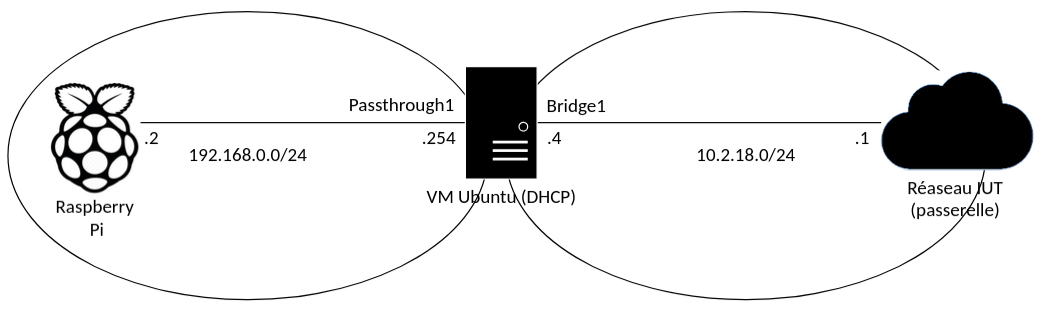
\includegraphics[scale=0.4]{rzo.png}
    \caption{Diagramme réseau simplifié de l'installation}
\label{fig:my_label}
\end{figure}
Le \acrshort{ah} est branché sur l'interface Passthrough1 de la \acrshort{vm}, pas de restriction quant au masque de sous-réseau ou les adresses choisies car étant un réseau local propre. L'adresse IP de la \acrshort{vm} sera considérée comme passerelle par les équipements de ce \gls{lan} (192.168.0.254 sera la passerelle du réseau 192.168.0.0/24).\\\\L'interface Bridge1 est reliée au réseau de l'IUT avec une adresse IP statique définie sur la plage d'adresses IP recommandée sur le poste utilisé. Ici en exemple .4, la plage d'adresse étant de 10.2.18.4 à 10.2.18.7 sur le poste TITI de la salle TP Réseaux sur lequel la configuration a été effectuée. Le \acrshort{ah} pourra communiquer avec les machines du réseau de l'IUT (10.2.18.0/24) et celles du \gls{wan} en plus de son \gls{lan} (192.168.0.0/24).
\begin{figure}[!ht]
    \centering
    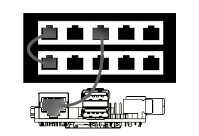
\includegraphics[scale=2]{poste.jpg}
    \caption{Branchements sur le panneau de raccordement du poste}
    \label{fig:poste}
\end{figure}
\begin{figure}[!ht]
    \centering
    
\includegraphics[scale=0.9]{baie2.png}
    \caption{Branchements sur la baie}
    \label{fig:baie}
\end{figure}
\newline
\newpage
\subsubsection{Illustration connexion capteur/Raspberry Pi}
\label{sec:branchementcapteur}
Le pin le plus à gauche du capteur vu de haut est appelé VCC, c'est-à-dire l'alimentation en +5V nécessaire que fournira le pin numéro 2 dit 5V PWR du \acrshort{ah}.\\\\Le deuxième pin du capteur est celui des données DATA rattaché à une résistance pull-up de 10 K Ohms (10 K Ohms étant la valeur de résistance maximale possible, 4.7 K Ohms la minimale). Ce pin est aussi placé sur celui \gls{gpio} 4 du \acrshort{ah} afin de récupérer les données (n'importe quel pin \gls{gpio} convient, voir schéma \hyperref[sec:fig5]{\textit{figure 5}}).\\\\Le quatrième et dernier pin du capteur est celui de la masse GND rattaché à celle du \acrshort{ah}.
\begin{figure}[!ht]
    \centering
    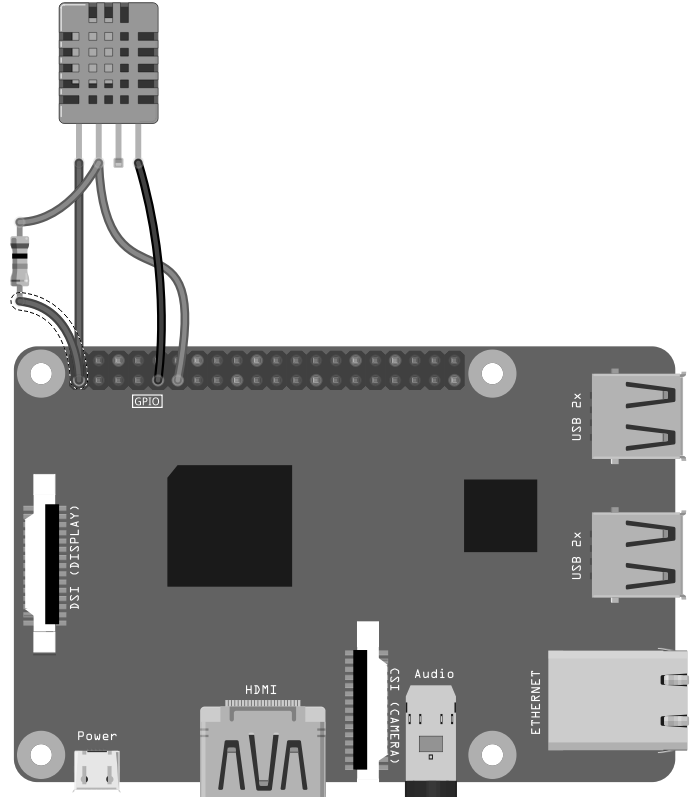
\includegraphics[scale=0.28]{grayscale_rpi1.png}
    \caption{Schéma des branchements du capteur DHT20 au RPI}
\end{figure}
\label{sec:fig5}
\begin{figure}[!ht]
    \centering
    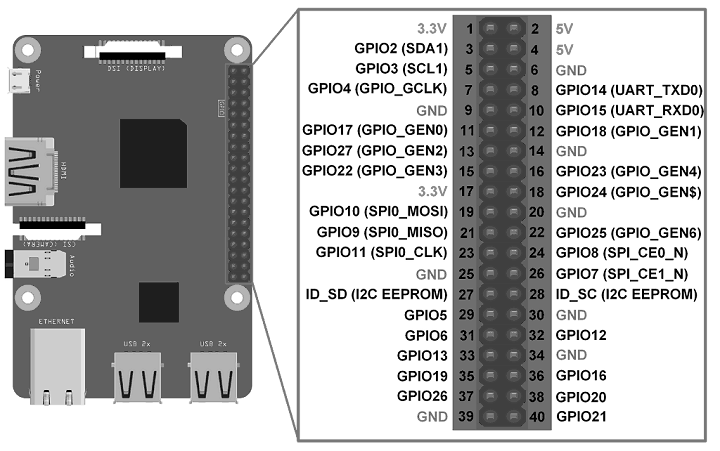
\includegraphics[scale=0.5]{gpio_pins_grayscale.png}
    \caption{Schéma des pins du RPI}
\end{figure}
\newpage
\section{Préparation du Raspberry Pi}
Le \acrshort{ah} sera configuré de manière "headless", c'est-à-dire sans périphérique d'entrée ou de sortie.\\\\Après l'avoir téléchargé, il faudra "installer" le SE sur l'emplacement reconnu de l'adaptateur de la carte micro SD. Une fois son installation effectuée, un utilisateur et un mot de passe seront assignés au SE. La configuration réseau sera vérifiée afin de permettre le bon fonctionnement de l'accès \gls{ssh}.
\subsection{Mise en place du système d'exploitation}
Il faut flasher, "installer" le SE une fois téléchargé pour ensuite configurer un utilisateur avec un mot de passe chiffré sur celui-ci.
\subsubsection{Récupération de l'image générique}
Pour ce cas d'usage, il est préférable de récupérer une image de \gls{rpios} allégé : \href{https://www.raspberrypi.com/software/operating-systems/}{\textit{Raspberry Pi OS Lite}}. Sa version Lite ne contenant pas d'environnement de bureau utilisera moins d'espace de stockage et de ressources matérielles (n'ayant pas les paquets pour et n'exécutant pas d'interface graphique utilisateur); en adéquation avec une utilisation headless.\\\\À l'emplacement du terminal, un fichier avec l'extension \verb|.iso| sera téléchargé et sera le fichier du \acrshort{se} avant son installation.
\definecolor{light-gray}{gray}{0.95}
\lstset{columns=fullflexible, basicstyle=\ttfamily,
    backgroundcolor=\color{light-gray},xleftmargin=0.5cm, xrightmargin=0.5cm,frame=tlbr,framesep=4pt,framerule=0pt,breaklines=true}
\begin{lstlisting}
    $ wget https://downloads.raspberrypi.org/raspios_lite_armhf/images/raspios_lite_armhf-2022-09-26/2022-09-22-raspios-bullseye-armhf-lite.img.xz
\end{lstlisting}
\subsubsection{Découverte de l'emplacement de stockage}
\label{sec:sec01}
Afin de flasher le fichier du système d'exploitation sur la carte micro SD du \acrshort{ah}, il faut connecter la carte micro SD sur la machine via l'adaptateur.\\\\Après cela reste à trouver la localisation du lecteur de la carte micro SD reconnu sur la machine.\\\\Affichage de l'emplacement des périphériques de stockage reconnus par le SE de la machine.
\begin{lstlisting}
    # lshw -C disk
\end{lstlisting}
\noindent Un exemple de sortie de cette commande, la micro SD de 32 Go reconnue sur \verb|/dev/sda|.
\begin{lstlisting}[language=bash]
  *-disk
       description: SCSI Disk
       product: SD/MMC/MS PRO
       vendor: Generic-
       physical id: 0.0.0
       bus info: scsi@1:0.0.0
       logical name: /dev/sda
       version: 1.00
       serial: 2012062914345300
       size: 29GiB (31GB)
       capabilities: removable
       configuration: ansiversion=4 logicalsectorsize=512 sectorsize=512
     *-medium
          physical id: 0
          logical name: /dev/sda
          size: 29GiB (31GB)
\end{lstlisting}
%  *-namespace:0
%       description: NVMe disk
%       physical id: 1
%       bus info: nvme@0:1
%       logical name: /dev/nvme0n1
%       size: 238GiB (256GB)
%       capabilities: gpt-1.00 partitioned partitioned:gpt
%       configuration: guid=a60f757c-dcfd-4648-b132-fcfdc5ba2205 
%       logicalsectorsize=512 
%       sectorsize=512 wwid=eui.01000000000000008ce38e0400a37168
\subsubsection{Installation de l'image sur la carte micro SD}
Après le téléchargement de l'image du \acrshort{se} à flasher ainsi que l'obtention de l'emplacement du périphérique de stockage, il faut écrire le contenu du fichier sur la carte micro SD.\\Le premier argument de la commande est le chemin vers le fichier en \verb|.iso| du \acrshort{se} lu, le terminal est ici à l'emplacement du fichier.\\\\La carte micro SD a comme emplacement \verb|/dev/sda| vu \hyperref[sec:sec01]{\textit{2.1.2}}.
\begin{lstlisting}
    # xzcat 2022-09-06-raspios-bullseye-armhf-lite.img.xz | dd bs=4M of=/dev/sda
\end{lstlisting}
\subsection{Configuration avant déploiement}
Un utilisateur avec un mot de passe chiffré seront affectés au SE du \acrshort{ah}. L'activation du service \gls{ssh} sera aussi effectué afin de pouvoir se connecter à distance au \acrshort{ah} avec cet utilisateur.
\subsubsection{Création d'un utilisateur avec son mot de passe}
\label{sec:sec03}
Afin de créer un utilisateur et un mot de passe personnalisés sur le \acrshort{ah}, il faut modifier un fichier de configuration du \acrshort{se} du \acrshort{ah}.\\\\Pour cela, d'abord débrancher et rebrancher l'adaptateur sur la machine après avoir flashé le SE afin que la carte micro SD soit reconnue comme un dispositif de stockage utilisable par la machine.\\\\Le contenu de la carte micro SD est reconnue sur le chemin d'accès \verb|/run/media/alexis/|, "alexis" le nom d'utilisateur de la session. L'emplacement et le contenu de la carte micro SD peuvent être observés dans l'explorateur de fichier du \acrshort{se} de la machine utilisé.\\Il faut ensuite modifier le fichier se trouvant dans /boot/userconf sur la carte micro SD, le chemin absolu de ce fichier dans ce cas sera donc \verb|/run/media/alexis/boot/userconf|.\\\\Afin d'éviter de fournir le mot de passe en clair, que celui-ci soit observable facilement à la lecture du fichier, la commande \verb|openssl| sera utilisé afin de générer un mot de passe chiffré dans le fichier de configuration des utilisateurs.\\\\Le mot de passe \verb|"tprzo.40"| sera attribué à l'utilisateur \verb|"alexispi"| dans le fichier\\\verb|/run/media/alexis/boot/userconf|.
\definecolor{light-gray}{gray}{0.95}
\begin{lstlisting}
    # echo "alexispi:"$(echo "tprzo.40" | openssl passwd -6 -stdin) > /run/media/alexis/boot/userconf
\end{lstlisting}
\subsubsection{Configuration réseau requise}
La configuration réseau initiale de \gls{rpios} repose sur l'attente d'une réponse \gls{dhcp} sur l'interface RJ45 Ethernet.\\\\Si besoin de configurer le \acrshort{ah} sur son interface Wi-Fi IEEE 802.11 lors du premier démarrage, il faudra configurer le fichier \verb|/etc/wpa_supplicant/wpa_supplicant.conf| présent sur la carte micro SD.\\\\Pour ce projet, il faut laisser le \acrshort{ah} se connecter sur le \gls{lan} via son interface RJ45 Ethernet, la \acrshort{vm} lui fournira la configuration réseau nécessaire sur cette interface via son service \gls{dhcp}.\\\\Pas de manipulation à faire sur la configuration réseau du \acrshort{ah} dans ce cas.
\subsubsection{Activation du service de connexion à distance}
\indent Le \gls{sh} du \acrshort{ah} sera accessible via une connexion \gls{ssh} depuis une machine cliente. Il faut indiquer au SE du \acrshort{ah} l'activation du service \gls{ssh} avant son déploiement.\\La création d'un fichier nommé \verb|ssh| dans le dossier \verb|/boot| de la carte micro SD suffit.\\\\L'emplacement du périphérique de stockage reste \verb|/run/media/alexis|.
\begin{lstlisting}
    $ touch /run/media/alexis/boot/ssh
\end{lstlisting}
\section{Déploiement d'un service DHCP}
Cette section présentera des explications et les configurations de base de la \acrshort{vm} afin de lui déployer un service \gls{dhcp}.
\subsection{Explications sur le service}
\label{sec:dhcpe}
Le service \gls{dhcp} donnera différentes informations aux nouveaux équipements arrivant sur le \gls{lan} qui émettent une requête afin de les obtenir.\\\\Le \gls{dhcp} distribuera les informations suivantes.
\begin{itemize}
    \item[•] L'adresse IP de la passerelle (192.168.0.254 ici)
    \item[•] Le masque de sous-réseau (/24 soit 255.255.255.0)
    \item[•] Les adresses IP des serveurs DNS (194.167.156.13 et 10.2.12.4)
    \item[•] Une adresse IP allouée pour l'interface de l'équipement
\end{itemize}
Un service \gls{dhcp} permet de ne pas avoir à renseigner manuellement toutes ces informations sur chaque appareil voulant se connecter sur un \gls{lan} et empêchera des conflits d'adresses IP par inadvertance.
\subsection{Création de la machine virtuelle}
L'outil de virtualisation pour créer une \acrshort{vm} Ubuntu sera \href{http://vi4rt.univ-pau.fr}{\textit{VI4RT}}.\\\\Les paramètres à ajouter sur la page \verb|Créer une machine| de VI4RT sont les suivants :
\begin{lstlisting}
    Nouvelle machine virtuelle

Nom de la machine: ubn1
Disque dur: Ubuntu 18.04 (15.00Go)
Processeur(s): 2 vcpus
Memoire vive: 4G
Cartes reseaux: 2
Carte 1 attachee a[...]: bridge1
Carte 2 attachee a[...]: pass1
\end{lstlisting}
Le \verb|Nom de la machine|, nombre de \verb|Processeur(s)| et de \verb|Mémoire vive| pouvant être modifiés, ceux indiqués étant à titre indicatifs.
\subsection{Configuration réseau de la machine virtuelle}
Il faut configurer les interfaces réseaux de la \acrshort{vm} avant de déployer le service \gls{dhcp}.
\subsubsection{Détection des interfaces réseaux}
\label{sec:secip}
\label{sec:sec02}
Il faut lister interfaces présentes sur la \acrshort{vm} avant de les configurer.\\
\begin{lstlisting}
    $ ip address
\end{lstlisting}
Un exemple de sortie de cette commande, ici sur la \acrshort{vm}.
\begin{lstlisting}    
    1: lo: <LOOPBACK,UP,LOWER_UP> mtu 65536 qdisc noqueue state UNKNOWN group default qlen 1000
    link/loopback 00:00:00:00:00:00 brd 00:00:00:00:00:00
    inet 127.0.0.1/8 scope host lo
       valid_lft forever preferred_lft forever
    inet6 ::1/128 scope host 
       valid_lft forever preferred_lft forever
2: ens3: <BROADCAST,MULTICAST,UP,LOWER_UP> mtu 1500 qdisc fq_codel state UP group default qlen 1000
    link/ether 52:54:00:95:5e:a8 brd ff:ff:ff:ff:ff:ff
    inet 10.2.18.4/24 brd 10.2.18.255 scope global ens3
       valid_lft forever preferred_lft forever
    inet6 2001:660:6701:30da:41e2:60b6:15a:5bce/64 scope global temporary dynamic 
       valid_lft 604515sec preferred_lft 85680sec
    inet6 2001:660:6701:30da:4316:b2a:a44c:28e0/64 scope global dynamic mngtmpaddr noprefixroute 
       valid_lft 2591879sec preferred_lft 604679sec
    inet6 fe80::e7dc:18bd:441b:2b9a/64 scope link noprefixroute 
       valid_lft forever preferred_lft forever
3: ens4: <BROADCAST,MULTICAST,UP,LOWER_UP> mtu 1500 qdisc fq_codel state UP group default qlen 1000
    link/ether 52:54:00:c7:c4:c3 brd ff:ff:ff:ff:ff:ff
    inet 192.168.0.254/24 brd 192.168.0.255 scope global ens4
       valid_lft forever preferred_lft forever
\end{lstlisting}
L'interface Bridge1 est reconnue comme étant \verb|ens3| et Passthrough1 sous \verb|ens4|, celles-ci correspondent aussi aux adresses MAC visibles sur la page de l'outil VI4RT si besoin de vérification.
\subsubsection{Configuration des interfaces réseaux}
L'un des utilitaires de gestions d'interfaces réseaux le plus répandu et utilisé se nomme \verb|NetworkManager|. Celui-ci est notamment présent sur les distributions Debian et Ubuntu comme gestionnaire de réseaux par défaut.\\\\Afin de le manipuler il est probant de modifier son fichier de configuration afin de définir les adresses IP, les masques de sous-réseaux ainsi que la passerelle souhaitée sur les interfaces de la \acrshort{vm}.\\\\Modification du fichier de configuration de NetworkManager sur la \acrshort{vm}.
\begin{lstlisting}
    # nano /etc/network/interfaces
\end{lstlisting}
En appliquant l'architecture de la \hyperref[sec:rzo]{\textit{figure 1}} avec les noms des interfaces vus \hyperref[sec:sec02]{\textit{3.3.1}}.
\begin{lstlisting}
auto ens3
iface ens3 inet static
    address 10.2.18.4
    netmask 255.255.255.0
    gateway 10.2.18.1
    
auto ens4
iface ens4 inet static
    address 192.168.0.254
    netmask 255.255.255.0
\end{lstlisting}
Application des paramètres aux interfaces via leur actualisation.
\begin{lstlisting}
    # ifup -a
\end{lstlisting}
\subsection{Installation du service}
Déploiement du service \gls{dhcp} sur la \acrshort{vm}. Celle-ci distribura les informations vues \hyperref[sec:dhcpe]{\textit{3.1}} aux machines en attentes de réponse \gls{dhcp} sur son interface \verb|ens4|.
\subsubsection{Mise à jour des paquets du système}
Avant d'installer un ou plusieurs paquets utilisant des fonctions systèmes, il est préférable de mettre à jour ces paquets.\\\\Installation des dernières versions disponibles des paquets du système.
\begin{lstlisting}
    # apt-get update -y && apt-get upgrade -y
\end{lstlisting}
Sur les \acrshort{vm} Ubuntu 18.04 sous VI4RT, la mise à jour des paquets systèmes installés ne peut directement s'effectuer : une erreur Glib de ce type étant remontée.
\begin{lstlisting}
(appstreamcli:12346): GLib-CRITICAL **: 12:15:21.490: g_variant_new_variant: 
assertion 'value != NULL' failed

(appstreamcli:12346): GLib-ERROR **: 12:15:21.490: g_variant_new_parsed: 
11-13:invalid GVariant format string
Trace/breakpoint trap
E: Problem executing scripts APT::Update::Post-Invoke-Success 'if /usr/bin/test 
-w /var/cache/app-info -a -e /usr/bin/appstreamcli; then appstreamcli 
refresh-cache > /dev/null; fi'
E: Sub-process returned an error code
\end{lstlisting}
Un correctif est possible en demandant la réinstallation du paquet \verb|libappstream4|. En suivant la mise à jour des paquets s'effectuera normalement.
\begin{lstlisting}
    # apt-get install --reinstall libappstream4 -y && apt-get update -y && apt-get upgrade -y
\end{lstlisting}
\subsubsection{Installation d'un paquet pour le service}
Ubuntu ne propose pas nativement un service réseau pouvant répondre aux attentes d'un serveur \gls{dhcp}, il faut installer un paquet adéquat.\\\\Un paquet intitulé \verb|is-dhcp-server| sera utilisé.
\begin{lstlisting}
    # apt-get install isc-dhcp-server -y
\end{lstlisting}
\subsection{Mise en place du service}
Le service \gls{dhcp} installé sera configuré afin de correspondre aux besoin du \gls{lan}.\\Avant de modifier les propriétés d'une interface, une sauvegarde sera effectuée afin d'éviter tous problèmes. La restauration de celle-ci sera montrée en cas de besoin.
\subsubsection{Sauvegarde du fichier de configuration vierge}
Le fichier avec le chemin absolu \verb|/etc/dhcp/dhcpd.conf| est le fichier de configuration du \gls{dhcp} après l'installation du paquet.\\\\Sa configuration est vide par défaut et est initialement prévu pour être modifié, celui-ci n'applique aucune règle si non configuré.
\newpage 
La sauvegarde sera une copie de la configuration vierge vers un autre fichier avec une extension \verb|.old|.
\begin{lstlisting}
    # cp /etc/dhcp/dhcpd.conf{,.old}
\end{lstlisting}
Si besoin de la restaurer, il faudra supprimer l'ancienne configuration utilisée par le service et renommer celle en \verb|.old| afin qu'elle reprenne sa place en lui retirant l'extension.\\\\Un redémarrage du service sera ensuite nécessaire afin que celui-ci puisse prendre en considération les modifications de ses règles.\\\\
\textbf{/!\textbackslash SI BESOIN DE RESTAURATION DE LA SAUVEGARDE}
\begin{lstlisting}
    # rm /etc/dhcp/dhcpd.conf; cp /etc/dhcp}/dhcpd.conf.old /etc/dhcp/dhcpd.conf; systemctl restart isc-dhcp-server
\end{lstlisting}
\subsubsection{Modification de la configuration du service}
Maintenant une copie de l'ancienne configuration de notre \gls{dhcp} vierge faite, il faut modifier la configuration active.\\\\La configuration du service \gls{dhcp} contiendra les instructions pour distribuer des adresses IP entre 192.168.0.1 et 192.168.0.253 aux arrivants sur le \gls{lan}. Plage d'adresses maximale pour le masque de sous-réseau et l'adresse de la passerelle  choisie, l'adresse en .254 étant choisie pour la \acrshort{vm} qui sera indiquée comme passerelle.\\\\Le \gls{dhcp} distribura aussi les adresses IP des serveurs DNS intérrogeables (194.167.156.13 et 10.2.12.4) en plus du masque de sous-réseau /24 (255.255.255.0). Les autres paramètres étant pour le temps par défaut et maximal accordés aux baux dynamiques alloués pour les adresses IP.\\\\Définition de ces paramètres dans le fichier \verb|dhcpd.conf|.
\begin{lstlisting}
    # nano /etc/dhcp/dhcpd.conf
\end{lstlisting}
Contenu du fichier \verb|/etc/dhcp/dhcpd.conf| après édition.
\begin{lstlisting}
default-lease-time 600;
max-lease-time 7200;
 
subnet 192.168.0.0 netmask 255.255.255.0 {
 range 192.168.0.1 192.168.0.253;
 option routers 192.168.0.254;
 option domain-name-servers 194.167.158.13, 10.2.12.4;
}
\end{lstlisting}
\subsubsection{Application et vérification de l'état du service}
Il faut maintenant appliquer les paramètres rentrés dans le fichier de configuration sur l'interface sur laquelle le service \gls{dhcp} sera actif.\\\\L'interface voulue est ici \verb|ens4|, celle sur Passthrough1.\\\\Information de l'interface dans le fichier ayant pour chemin absolu \verb|/etc/default/isc-dhcp-server|.
\begin{lstlisting}
    # nano /etc/default/isc-dhcp-server
\end{lstlisting}
Fichier après l'édition.
\begin{lstlisting}
    INTERFACESv4="ens4"
\end{lstlisting}
Suite à l'application des paramètres il faut vérifier que le service soit bien actif et que celui-ci ne reporte pas d'erreur.\\\\Si la sortie de la commande suivante renvoie en vert un message \verb|active (running)|, alors le service a redémarré et a appliqué les paramètres renseignés. Sinon des instructions ou message(s) d'erreur(s) seront indiqué(s).\\\\Utilisation de la commande \verb|systemctl| (Q ou CTRL+C pour quitter) afin de regarder le status du service \gls{dhcp}.
\begin{lstlisting}
    # systemctl restart isc-dhcp-server; systemctl status isc-dhcp-server
\end{lstlisting}
Suite à celà, si le \acrshort{ah} est connecté sur l'interface Passthrough1 de la \acrshort{vm}, celui-ci intégrera le \gls{lan} suivant le masque de sous-réseau avec une adresse IP permise depuis la plage d'adresses accordée au \gls{dhcp}. Celui-ci aura aussi configuré son interface avec deux serveurs DNS interrogeables ainsi que l'adresse IP de la \acrshort{vm} en tant que passerelle du \gls{lan}.
\section{Configuration d'un NAT}
Afin que les équipements du \gls{lan} puissent communiquer avec ceux des autres réseaux, il faut configurer un routeur \gls{nat} qui s'occupera de faire traverser les paquets IP et de faire correspondres les adresses aux bons destinataires de chaques réseaux.
\subsection{Explications sur le routage d'adresses et de paquets}
La \acrshort{vm} fera circuler les requêtes et réponses IP des équipements connectés sur le \gls{lan} aux réseaux accessibles par son autre interface (ens3 Bridge1) et inversement. En d'autres termes la \acrshort{vm} fera accéder le \acrshort{ah} au \gls{wan} et au réseau de l'IUT, ses requêtes et les réponses attendues pour des réseaux extérieurs sortant du \gls{lan} pour revenir vers lui par la \acrshort{vm}.\\La \acrshort{vm} translatera les adresses IP entre les réseaux et fera de la redirection de paquets sur ses interfaces en conséquence.\\\\Si les équipements du \gls{lan} comme le \acrshort{ah} avaient eu uniquement besoin de communiquer avec d'autres équipements du réseau local, la redirection de paquets et d'adresses n'auraient pas été nécessaires.\\\\À noter que le \acrshort{ah} aura accès au \gls{wan} uniquement car la \acrshort{vm} a la possibilité de le faire via le réseau de l'IUT et sa passerelle.
\subsection{Paramètrage de la redirection d'adresses}
L'activation du \gls{nat} passe par l'autorisation des redirections du trafic IP sur les interfaces de la \acrshort{vm}. Ce procédé appelé \gls{ipforward} permet de faire circuler les paquets voulus sur le bon réseau pour peu que l'adresse de destination du paquet soit accessible par la \acrshort{vm}.
\subsubsection{Activation de la variable de routage}
L'activation du \gls{nat} est contingent à l'activation d'une variable système sur la \acrshort{vm} afin de faire circuler les paquets IP d'un réseau à un autre. Cette variable se nomme \verb|ip_forward| décrite précédemment, l'activation s'effectue en changeant sa valeur à 1, initialement 0 non actif.\\\\Activation du routage des paquets IP.
\begin{lstlisting}
    # sysctl -w net.ipv4.ip_forward=1
\end{lstlisting}
\subsubsection{Application de la redirection sur l'interface}
Il faut désormais définir sur quelle interface l'ip foward devra être actif.\\\\Pour ce cas il faut définir l'\gls{ipforward} sur l'interface Bridge1 soit ens3 la \acrshort{vm} afin que les requêtes du \gls{lan} puisse accéder au réseau local de l'IUT ainsi qu'au \gls{wan} et inversement. La commande précise aussi quoi rediriger en créant une couche NAT afin de relier les deux réseaux.\\\\Définition de l'\gls{ipforward} sur l'interface ens3 de notre \acrshort{vm} via un NAT.
\begin{lstlisting}
    # iptables -t nat -A POSTROUTING -o ens3 -j MASQUERADE
\end{lstlisting}
\subsection{Contrôles supplémentaires après configuration}
\label{sec:ici}
L'installation terminée, en cas de problème ou de conflit quelques vérifications simplessont possibles afin de vérifier l'intégrité de l'infrastructure.\\\\Ces vérifications sont optionnelles et sont mises à disposition selon les besoins.
\subsubsection{Vérification des adresses}
Il est préférable de vérifier les adresses IP des interfaces des équipements afin de s'assurer de leur identification sur les différents réseaux.\\\\Affichage des adresses IP des interfaces d'un équipement.
\begin{lstlisting}
    $ ip address
\end{lstlisting}
Un exemple de sortie de cette commande est proposé \hyperref[sec:secip]{\textit{3.3.1}} pour la \acrshort{vm}.
\subsubsection{Vérification des routes des appareils}
Si un problème lors des tentatives de communications, on peut vérifier la route que doivent prendre les paquets IP sur les différents appareils.\\\\Affichage du chemin des paquets d'une machine selon l'adresse de destination.
\begin{lstlisting}
    $ ip route
\end{lstlisting}
Exemple de la sortie de la commande sur la \acrshort{vm}.
\begin{lstlisting}
    default via 10.2.18.1 dev ens3 onlink 
    10.2.18.0/24 dev ens3 proto kernel scope link src 10.2.18.4 
    192.168.0.0/24 dev ens4 proto kernel scope link src 192.168.0.254 
\end{lstlisting}
\section{Connexion et manipulations du Raspberry Pi}
Maintenant l'infrastructure réseau opérationnelle, il faut initier une connexion \gls{ssh} au \acrshort{ah} et utiliser le capteur rattaché suivant sa localisation sur le réseau et les branchements du capteur.
\subsection{Connexion et débuts de communications}
Il faut intier une connexion \gls{ssh} sur le \acrshort{ah} définit comme hôte. Afin d'atteindre la machine attendue en \gls{ssh} il faut renseigner soit l'adresse IP de la machine à joindre soit le nom d'hôte sur le réseau \verb|hostname|.\\\\Le mot de passe de l'utilisateur sera demandé une fois la connexion initiée.
\subsubsection{Recherche de l'appareil sur le réseau}
\label{sec:iprpi}
Afin de pouvoir initier une connexion au \acrshort{ah}, il faut connaitre son accessibilité sur le \gls{lan} et son emplacement - adresse IP.\\\\Pour cela une requête \gls{icmp} suffit afin d'essayer de le joindre sur le réseau local.\\\\Cependant, ne connaissant pas l'adresse IP que le \gls{dhcp} a attribué au \acrshort{ah}, il est probant d'envoyer une requête \gls{icmp} aux machines du \gls{lan} et voir laquelle ou lesquelles sont accessibles.\\Cette manipulation est possible en connaissant de l'adresse réseau et du masque de sous-réseau appliqué.\\\\Envoie de requêtes \gls{icmp} sur les machines du \gls{lan} via la commande \verb|ping|, exclue .254 la \acrshort{vm}, .255 le broadcast et .0 l'adresse réseau.
\begin{lstlisting}
    $ for ip in $(seq 1 253); do ping -c 1 -W 1 192.168.1.$ip | grep "ttl"; done
\end{lstlisting}
La sortie de commande renvera les pings réussi sur le \gls{lan}. Une adresse IP ou plus seront affichées, l'une correspondant à celle du \acrshort{ah} attribuée par le \gls{dhcp}, les autres pouvant être d'autres machines du réseau local. 
\begin{lstlisting}
    64 bytes from 192.168.0.253: icmp_seq=1 ttl=64 time=3.72 ms
\end{lstlisting}
L'adresse \verb|192.168.0.253| a été ici attribuée au \acrshort{ah} par le \gls{dhcp}, de plus celui-ci est joignable par la machine ayant initiée le ping.\\Si le \verb|ping| n'arrive pas à joindre le \acrshort{ah}, il est probant de vérifier la configuration réseau de la \acrshort{vm} et du \acrshort{ah} vu \hyperref[sec:ici]{\textit{4.3}}.\\\\Une autre méthode afin de trouver le \acrshort{ah} sur le réseau consiste à analyser le fichier d'attribution des adresses IP du serveur \gls{dhcp}.\\Préférez quand même la première méthode pouvant être effectuée depuis n'importe quelle machine du \gls{lan}, la deuxième necéssitant d'être effectuée depuis le serveur \gls{dhcp} ou de pouvoir accéder à ses fichiers.
\begin{lstlisting}
    $ cat /var/lib/dhcp/dhcpd.leases
\end{lstlisting}
Exemple de sortie de commande du fichier d'attribution des adresses du serveur \gls{dhcp}.
\begin{lstlisting}
    lease 192.168.0.253 {
      starts 3 2022/12/21 08:32:45;
      ends 3 2022/12/21 08:42:45;
      cltt 3 2022/12/21 08:32:45;
      binding state active;
      next binding state free;
      rewind binding state free;
      hardware ethernet dc:a6:32:05:7f:05;
      uid "\001\000\014)\262|\267";
      client-hostname "raspberrypi";
    }
\end{lstlisting}
L'usage d'outil d'analyse réseau comme nmap ou fping aurait aussi pu être fait mais non disponible nativement sur Ubuntu 18.04 comme voulu dans le préambule.
\subsubsection{Initialisation d'une connexion au Raspberry Pi}
En connaissance de l'adresse IP du \acrshort{ah}, il faut désormais initier une connexion \gls{ssh} sur celui-ci.\\\\La connexion se ferra avec l'utilisateur "alexispi" configuré \hyperref[sec:sec03]{\textit{2.2.1}} sur l'adresse IP vue \hyperref[sec:iprpi]{\textit{5.1.1}}.\\\\Initialisation d'une connexion \gls{ssh} sur le \acrshort{ah}.
\begin{lstlisting}
    $ ssh alexispi@192.168.0.1
\end{lstlisting}
Le mot de passe de l'utilisateur renseigné sera demandé, le \gls{sh} du \acrshort{ah} sera retranscrit sur la machine cliente ensuite. 
\subsection{Utilisation du capteur}
Le capteur permettra de récupérer l'humidité et la temprérature ambiantes si correctement branché. Rattaché au \acrshort{ah}, celui-ci interprêtera ses valeurs afin de les retranscrire.
\subsubsection{Explications sur l'utilisation du capteur}
Afin de récupérer ces données il faut connecter le capteur au \acrshort{ah}, branchement présents \hyperref[sec:branchementcapteur]{\textit{1.2.2}}.\\Un programme Python récupérera et interprétera les données reçues du capteur afin que l'on puisse les comprendre.
\subsubsection{Programme Python pour utiliser le capteur}
Les phrases initées par des hashtags sont des commentaires afin de mieux comprendre les lignes du programme.
\begin{lstlisting}[language=iPython]
import time, board, adafruit_dht

dht_device = adafruit_dht.DHT22(board.D4) # Charge le capteur sur le PIN GPIO 4

while True:
    try:
        temperature, humidity = dht_device.temperature, dht_device.humidity 
        # Recupere les donnees du capteur
        
        print("Temperature: " + str(temperature) + " C, Humidite: " + str(humidity) + "%", end="\r") 
        # Affiche les donnees sur la console
        
    except RuntimeError:                          # Prevention contre donnees du capteur corrompues 
        time.sleep(2.0)                             # Pause de 2 secondes
        continue                                     # Reprise de la boucle
        
    except Exception as error:                  # Precaution contre erreur grave extremement rare
        dht_device.exit()                          # Ferme proprement la liaison capteur-programme si erreur
        raise error                                  # Laisse l'erreur interrompre le programme
        
    time.sleep(2.0)                                 # Raffraichissement toutes les 2 secondes 
\end{lstlisting}
Exemple de sortie du programme.
\begin{lstlisting}
    Temperature: 24.2 C, Humidite: 57.7%
\end{lstlisting}
\end{document}